% Franklin's involution: 7+6+5+2 (slope 3, smallest part 2) and 8+7+5. Generated by a short script.
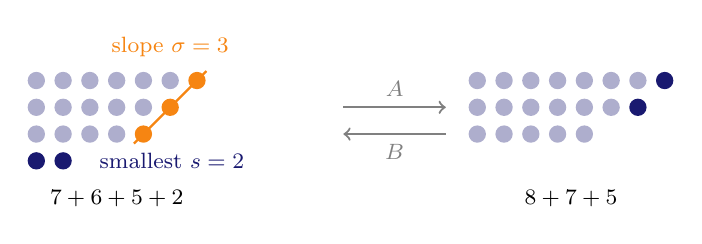
\begin{tikzpicture}[every node/.style={font=\footnotesize}]
\fill[MidnightBlue!35] (0.000,0.000) circle (0.11);
\fill[MidnightBlue!35] (0.340,0.000) circle (0.11);
\fill[MidnightBlue!35] (0.680,0.000) circle (0.11);
\fill[MidnightBlue!35] (1.020,0.000) circle (0.11);
\fill[MidnightBlue!35] (1.360,0.000) circle (0.11);
\fill[MidnightBlue!35] (1.700,0.000) circle (0.11);
\fill[BurntOrange] (2.040,0.000) circle (0.11);
\fill[MidnightBlue!35] (0.000,-0.340) circle (0.11);
\fill[MidnightBlue!35] (0.340,-0.340) circle (0.11);
\fill[MidnightBlue!35] (0.680,-0.340) circle (0.11);
\fill[MidnightBlue!35] (1.020,-0.340) circle (0.11);
\fill[MidnightBlue!35] (1.360,-0.340) circle (0.11);
\fill[BurntOrange] (1.700,-0.340) circle (0.11);
\fill[MidnightBlue!35] (0.000,-0.680) circle (0.11);
\fill[MidnightBlue!35] (0.340,-0.680) circle (0.11);
\fill[MidnightBlue!35] (0.680,-0.680) circle (0.11);
\fill[MidnightBlue!35] (1.020,-0.680) circle (0.11);
\fill[BurntOrange] (1.360,-0.680) circle (0.11);
\fill[MidnightBlue] (0.000,-1.020) circle (0.11);
\fill[MidnightBlue] (0.340,-1.020) circle (0.11);
\draw[BurntOrange,thick] (2.160,0.120)--(1.240,-0.800);
\node[BurntOrange,anchor=south] at (1.700,0.180) {slope $\sigma=3$};
\node[MidnightBlue,anchor=west] at (0.680,-1.020) {smallest $s=2$};
\node at (1.020,-1.496) {$7+6+5+2$};
\fill[MidnightBlue!35] (5.600,0.000) circle (0.11);
\fill[MidnightBlue!35] (5.940,0.000) circle (0.11);
\fill[MidnightBlue!35] (6.280,0.000) circle (0.11);
\fill[MidnightBlue!35] (6.620,0.000) circle (0.11);
\fill[MidnightBlue!35] (6.960,0.000) circle (0.11);
\fill[MidnightBlue!35] (7.300,0.000) circle (0.11);
\fill[MidnightBlue!35] (7.640,0.000) circle (0.11);
\fill[MidnightBlue] (7.980,0.000) circle (0.11);
\fill[MidnightBlue!35] (5.600,-0.340) circle (0.11);
\fill[MidnightBlue!35] (5.940,-0.340) circle (0.11);
\fill[MidnightBlue!35] (6.280,-0.340) circle (0.11);
\fill[MidnightBlue!35] (6.620,-0.340) circle (0.11);
\fill[MidnightBlue!35] (6.960,-0.340) circle (0.11);
\fill[MidnightBlue!35] (7.300,-0.340) circle (0.11);
\fill[MidnightBlue] (7.640,-0.340) circle (0.11);
\fill[MidnightBlue!35] (5.600,-0.680) circle (0.11);
\fill[MidnightBlue!35] (5.940,-0.680) circle (0.11);
\fill[MidnightBlue!35] (6.280,-0.680) circle (0.11);
\fill[MidnightBlue!35] (6.620,-0.680) circle (0.11);
\fill[MidnightBlue!35] (6.960,-0.680) circle (0.11);
\node at (6.790,-1.496) {$8+7+5$};
\draw[->,thick,gray] (3.9,-0.340)--(5.2,-0.340) node[midway,above] {$A$};
\draw[<-,thick,gray] (3.9,-0.680)--(5.2,-0.680) node[midway,below] {$B$};
\end{tikzpicture}
